\chapter{Data Analysis} \label{Chapter5}

\section{SQ1: What data types, available from the control system, can predict maintenance activities?} \label{SQ1}
How the different types of data can be extracted from the RAC's is explained in Section \ref{Data Gathering}. For every type of data that can be collected, it have to be determined if it is able to predict failures and therefore upcoming maintenance. Firstly, to understand what type of data should be collected and analyzed, it have to be determined which components from a robot arm require most costly maintenance. Cheap components or components that are easy to replace will not be considered since there is little to gain. Therefore, the CBM tool should focus at components that are costly or time-consuming to maintain and repair. From interviews with OTD employees and the Maintenance Engineer it is determined that the components within a robot arm joint are most time-consuming and costly to repair or replace. Therefore, this research will focus on these type of maintenance activities. Secondly, it have to be determined what data types are able to predict abnormality in robot arms and can be used to provide robot condition estimations. 

\subsection{Failure modes} \label{Failure modes}
In the maintenance logbook from Philips, all maintenance activities/event logs from 2011 to present are listed. In Figure \ref{fig:Cobra joint failures} it can be seen how many failures and events are related to which joint of a robot arm. Only the failures regarding Cobra s600s and s800s are included since those arms are similar and used mostly. In total, 97 major robot arm joint failures occurred and replacement was necessary. The number of failures per joint are 22, 64, 6, and 3 for joints 1, 2, 3, and 4, respectively. This is depicted in Figure \ref{fig:Cobra joint failures}. For most robot arms at Philips joint 1 and 2 are the joints with the highest average speed and torque and therefore it is assumed that joints with high speed and torque are more likely to fail. For this reason, data available from the joint of a robot arm with the highest average speed and torque will be focused on. 

Furthermore, the maintenance logbook shows that most failures are related to harmonic drive and motor failure. In total, 110 components were replaced where the motor and the harmonic drive caused failure mostly. The number of replaced components is higher than the number of failures since some failures required maintenance on multiple components. The number of failures per joint component is depicted in Figure \ref{fig:Joint failure component}. According to mechanics at Philips, motors and harmonic drives are replaced simultaneously and failure of a harmonic drive is the reason that a motor fails. Oil from a broken harmonic drive leaks through the motor and causes it to fail. 
\begin{figure}[ht]
\begin{subfigure}{.5\textwidth}
\centering
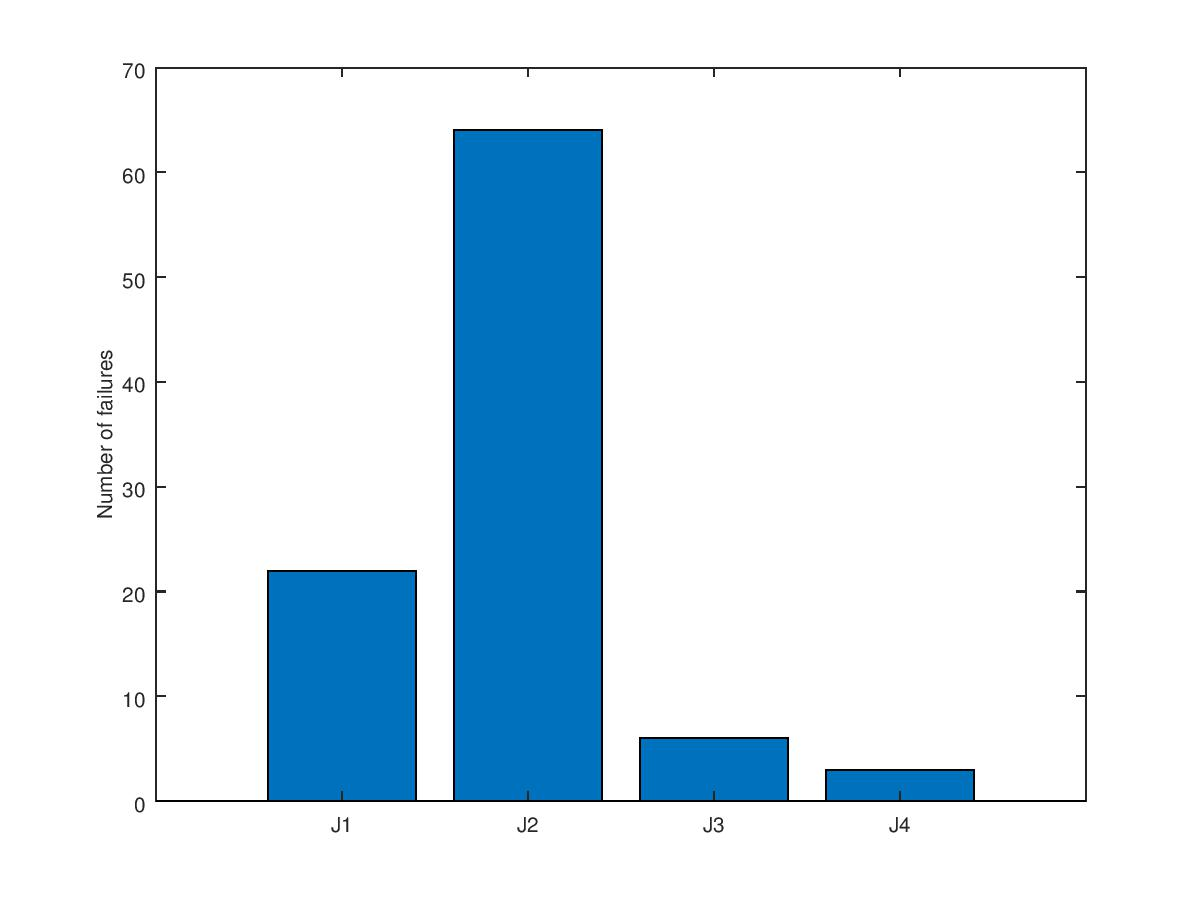
\includegraphics[width=.9\linewidth]{Figures/Cobra_joint_failures}
\caption[Number of Cobra s600/s800 joint failures]{Number of Cobra s600/s800 joint failures}
\label{fig:Cobra joint failures}
\end{subfigure}
\begin{subfigure}{.5\textwidth}
\centering
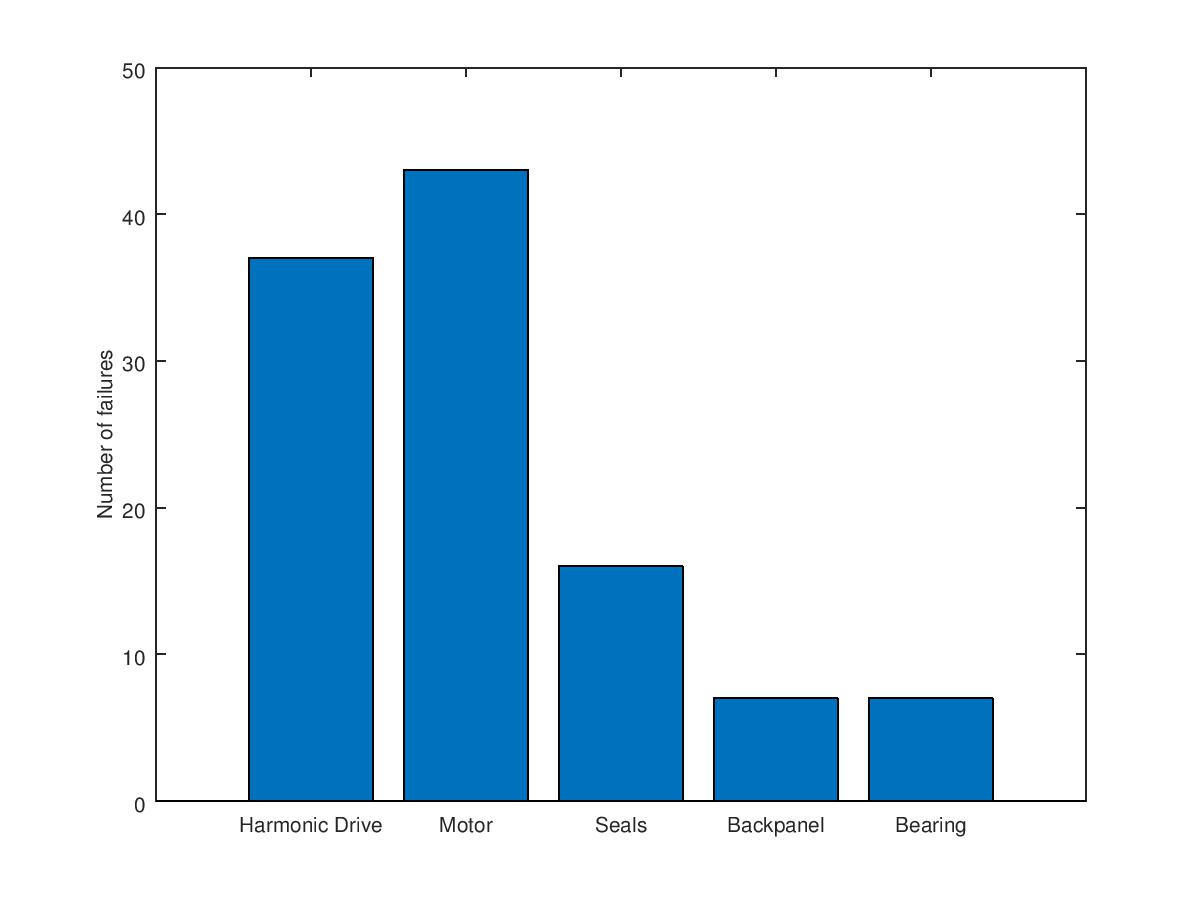
\includegraphics[width=.9\linewidth]{Figures/Joint_failure_component}
\caption[Number of failures per joint component]{Number of failures per joint component}
\label{fig:Joint failure component}
\end{subfigure}
\caption[Failure modes]{Robot arm failure modes. ({\tiny{A}}) Shows the number of failures that occurred at corresponding joints. ({\tiny{B}}) shows the components within a joint where a failure occurred.}
\label{fig:Failure data}
\end{figure}
As described in Section \ref{Hardware}, the harmonic drive of a Cobra s600 is exposed to wear and fatigue elements due to friction within the components. If the friction within a harmonic drive can be determined, an estimation of the component condition can be given and a RUL can be estimated. Friction is dependent on the contact geometry, topology, properties of the materials, relative velocity, lubricant, etc. \parencite{Al-Bender2008}. According to \citet{Bittencourt2012}, the following factors will be more or less significant to the total friction:
\begin{multicols}{2}
\begin{itemize}
\item temperature,
\item force/torque levels,
\item position,
\item velocity,
\item acceleration,
\item lubricant properties.
\end{itemize}
\end{multicols} 

\subsection{Relevant data} \label{Relevant data}
Based on the statements from the previous section, data available from the data collection methods, described in Section \ref{Data Gathering}, will be investigated on their relevance. According to the Adept User's Guide, force/torque levels are proportional to DC input voltages. Furthermore, the position error of a joint, the difference between the commanded position and the actual position, can be used to determine robot arm accuracy. As mentioned before, lubricant properties and temperature can also indicate robot failure. However, it is difficult to analyze lubricant continuously and will therefore not be investigated.

\subsubsection{DC Input Voltage} \label{DC Input Voltage}
The electric motor drives use power transistors to deliver energy. These transistors produce voltage; current is generated by the electrical circuit that is formed from the drive voltage and the motor windings. Because the power transistors produce voltage, a current loop is required to achieve precise control of current. A current loop compares the current command to the feedback and adjusts the drive voltage to minimize the error. 

\citet{Rajagopalan2006} proved theoretically and validated experimentally that faults in gears coupled to electric motors can be detected by monitoring either the voltage or the current in the motor driving the gear. Within their experiments they tested three types of gear faults: i) damaged gear tooth (local-tooth fault - deformation in one or two teeth), ii) scoring (loss of lubrication), and iii) debris in lubricant. They further describe that abnormality in an electric motor should appear in the stator voltage because a current-controlled motor should have no-stator-current harmonics as the motor current is regulated to the reference value. This indicates that when a motor of a Cobra s600 shows abnormality in voltage, it is related to abnormality in the applied torque. Data collection from a new assembly line, with the Adept ACE software, showed that the the voltage and current applied to the amplifier are oscillating around certain values. During motion, the DC input voltage is changing according to the commanded position. This can be seen in Figure \ref{fig:Electric Values}, where the commanded position and the corresponding voltage are depicted from a Cobra s600 during operation. When a negative position is required, the input voltage decreases and when a positive position is required, the input voltage increases. As mentioned above, abnormality in the input voltage is related to abnormality in applied torque. This indicates that analyzing DC input voltage can be used to predict abnormal behavior of a robot arm. However, the data is collected by the Data Collection Tool, as described in Section \ref{Data Gathering}, with a frequency of 1000 Hz. This function is not available on assembly lines with the Adept Desktop software and hence, other types of data will be analyzed so that a model can be designed which is useful for Adept ACE and Adept Desktop software. 
\begin{figure}[ht]
\centering
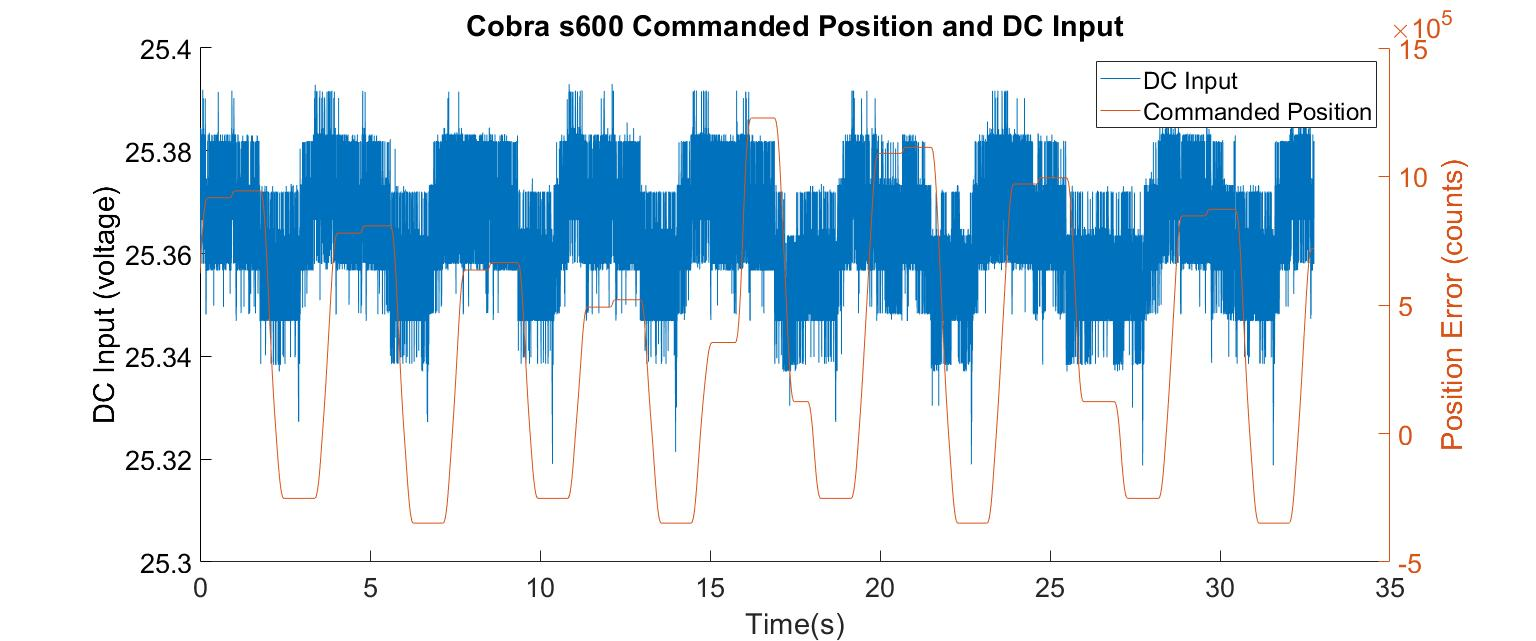
\includegraphics[width=\textwidth]{Figures/ComPosDCIn20}
\caption[DC Input voltage and Commanded Position for Cobra s600]{DC Input voltage and Commanded Position for Cobra s600} \label{fig:Electric Values}
\end{figure}

\subsubsection{Temperature} \label{Temperature}
As mentioned in Section \ref{Failure modes}, a changing temperature of a motor can also indicate failure. The robot arm joint motors are not equipped with temperature sensors. However, the encoder, located inside the robot arm joint motors, is equipped with a temperature sensor. When the temperature of a motor increases, the temperature of the encoder will increase as well.

To investigate if the encoder temperature can indicate robot joint failure, the daily average encoder temperatures from faulty and normal operating robot joints are reviewed. In Figure \ref{fig:AvgEncTemp}, it can be seen that faulty robot joints have, on average, a higher encoder temperature. This can indicate that the temperature of the corresponding motor is higher at faulty robot joints than normal operating joints. However, there are other causes that explain encoder temperature differences. The encoder can translate the robot joint position to the controller and does this by measuring the traveled distance of a joint motor. When this distance is large and/or the speed is high, the temperature of the encoder is increased. This indicates that a high encoder temperature is not only related to the motor temperature but also to the traveled distance and speed. To research whether the encoder temperature can indicate motor failure, monitoring the temperature values will be continued daily. 
\begin{figure}[ht]
\centering
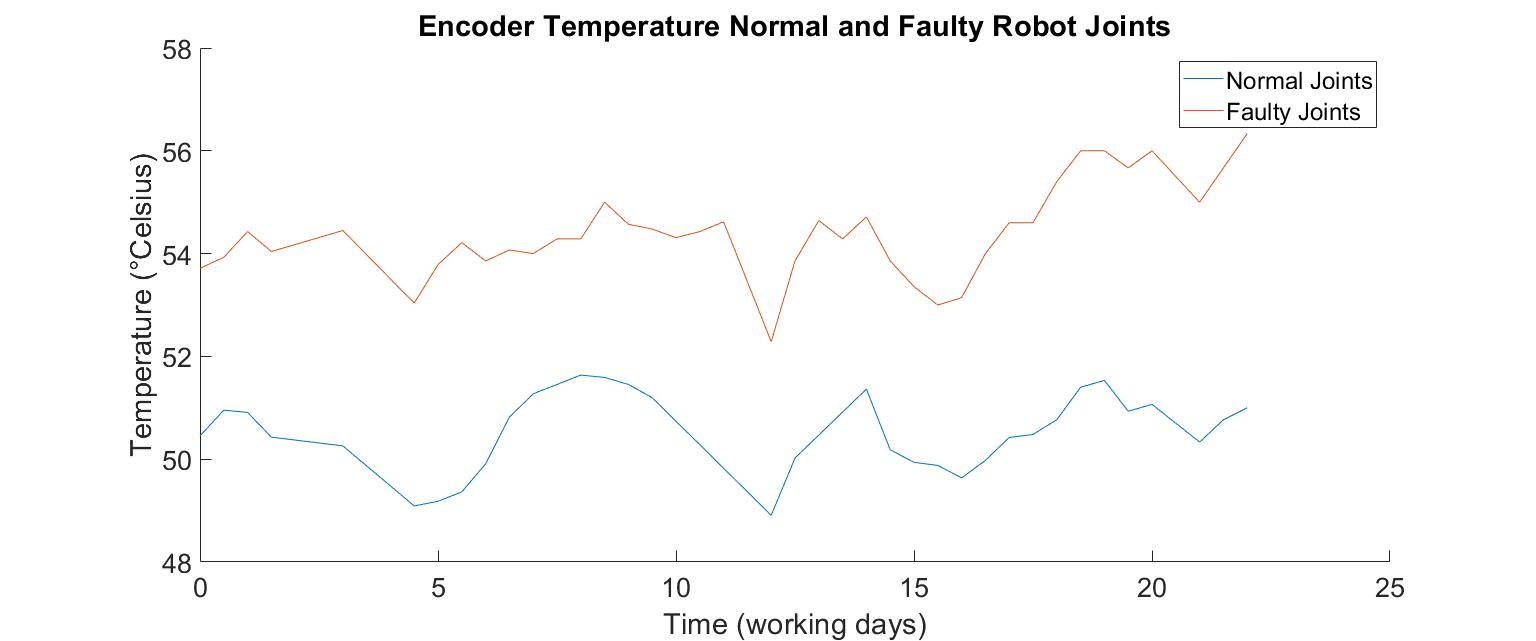
\includegraphics[width=\textwidth]{Figures/EncTemperatures}
\caption[Average encoder temperatures of normal and faulty robot arms]{Average encoder temperatures of normal and faulty robot arms} \label{fig:AvgEncTemp}
\end{figure}

According to the statements above, it is not yet conclusive that encoder temperature can indicate robot joint failure. Therefore, monitoring the temperature values will be continued daily. Afterwards, when it can be proven that encoder temperature, and perhaps more variables, can indicate robot joint failure, the model can be adjusted with implementing those variables. A Principal Component Analysis (PCA) can be useful to reduce the number of variables that are related to each other in the obtained data. It is a powerful tool for reducing the number of variables that can account for most of the variance in the data set \parencite{Virk2012}.

\subsubsection{Position Error} \label{Position Error}
As mentioned before, the position error of a robot arm joint is the difference between the commanded position and the actual position of that specific joint, also called robot joint accuracy. Once the controller receives a new input task, it have to send a commanded position to the corresponding amplifier which it then tries to reach. The height of the position error is related to the speed of the joint and the load applied to that joint. A higher speed and/or a heavier load will increase the position error \parencite{Qian1996}. According to \citet{Qiao2017} The consideration of robot joint accuracy is one of the key elements when assessing the health state of an industrial robot.

To investigate if the position error can indicate robot arm abnormality, the position errors of a proper working and a faulty robot arm are collected. The position error from the two Cobra s600's are depicted in Figure \ref{fig:HighFreqPosError}, where RA41 is the proper and RB72 is the faulty robot arm. The position errors are obtained at 1000 kHz by using the ACE software as explained in Section \ref{Software}. It can be seen that the position error peaks from RB72 are much higher than the peaks regarding RA41. The peak position error data is the highest position error that occurred since the controller is switched on. Therefore, it can occur that a peak position error has the same value as at the previous inspection.

As mentioned before, a robot arm with a higher operating speed will have higher position error peaks. It can occur that a faulty robot arm has lower position error peaks than a proper working robot arm. In other words, every robot arm has a different failure level. This failure level should therefore be threated as a variable within the intended model.
\begin{figure}[ht]
\centering
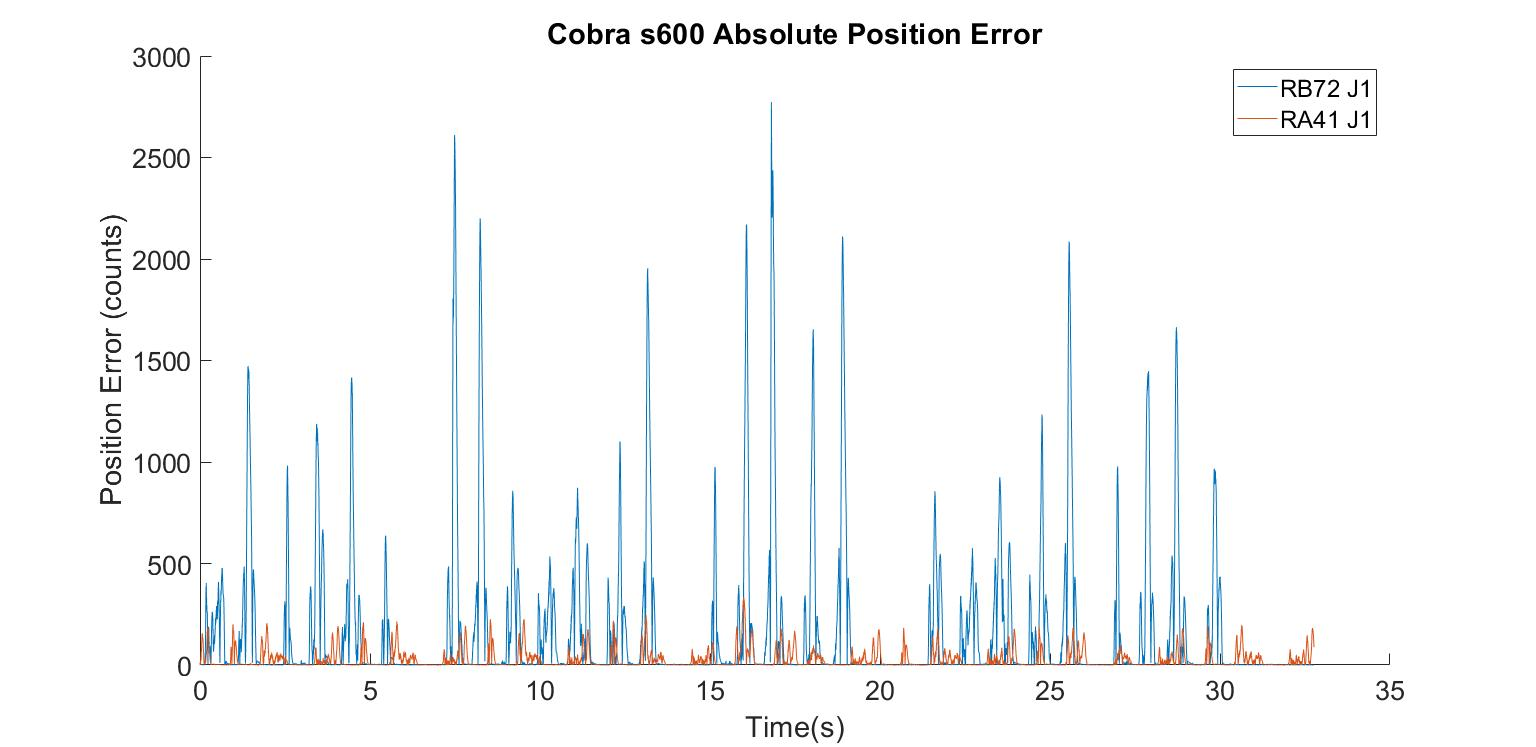
\includegraphics[width=\textwidth]{Figures/HighFreqError20}
\caption[Absolute position error for Cobra s600]{Absolute position error for Cobra s600} \label{fig:HighFreqPosError}
\end{figure}

In Figure \ref{fig:AllPosErrors}, the peak position error from several Cobra s600 robot arms are depicted. Since, the robot arms are only operating from Monday to Friday, the weekends are left out. The total time of the figure is from March 1 to March 30, or 21 working days. The red crosses indicate when a robot arm failed and was replaced by a new or revised one. As can be seen in the figure, failure at RB34 R2 J1 occurred at a lower peak position error than the failure at RB72 R1 J1. This indicates that the critical failure level differs per robot arm and a variable failure threshold should be considered. 
\begin{figure}[ht]
\centering
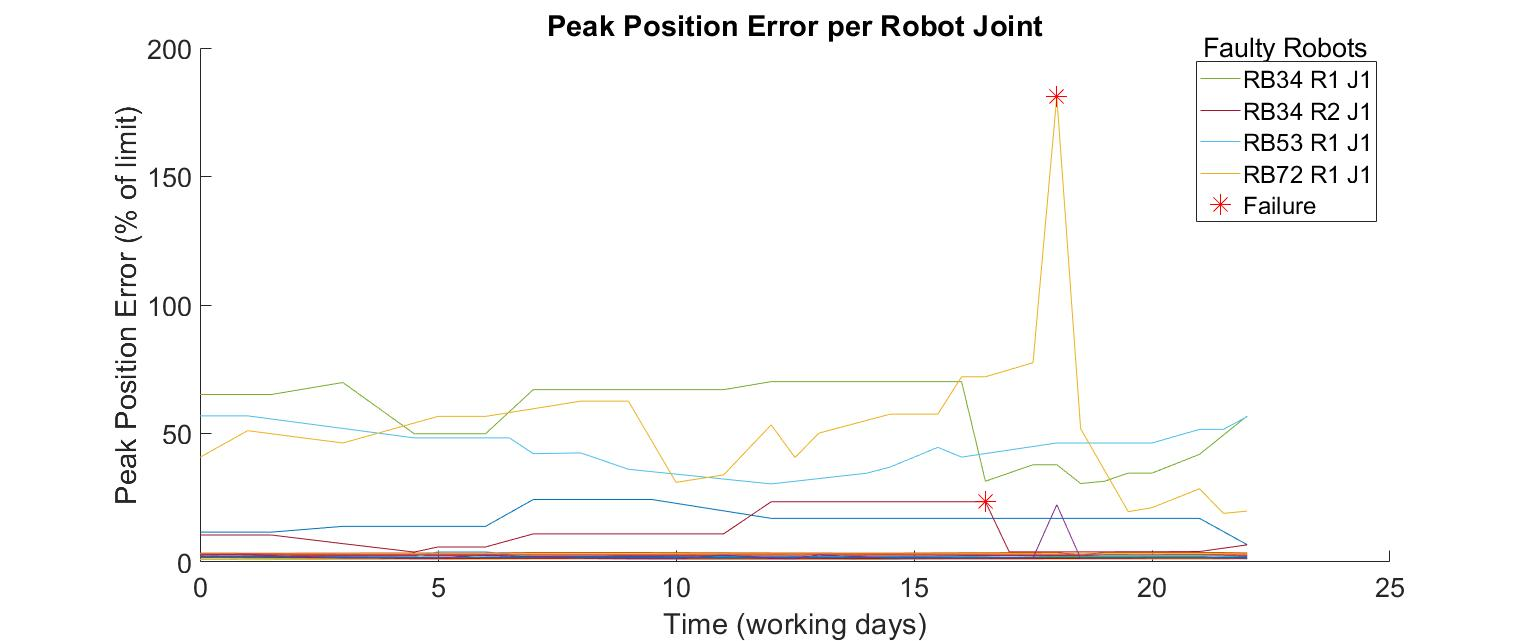
\includegraphics[width=\textwidth]{Figures/AllPeakPositionErrors20}
\caption[Peak position errors for several Cobra s600 robot arms]{Peak position errors for several Cobra s600 robot arms} \label{fig:AllPosErrors}
\end{figure}

\section{SQ2: How can the output data be interpret in order to predict maintenance?} \label{SQ2}
In the previous subsection, it was found that position error data is able to predict upcoming maintenance. Therefore, actual position error data is used to determine the path of degradation per robot arm joint. Based on this degradation path it can be predicted when the degradation has reached a critical failure level. In Figure \ref{fig:DegradationDistribution} it can be seen how the failure time should be estimated. From the known degradation path, the path left of $t$, a prediction can be achieved to determine how the degradation will evolve. The evolution of the degradation path is estimated and therefore the time to failure is also an estimate. Since that the position error data includes negative values a normal distribution for the time to failure estimation is considered. The distribution parameters, mean ($\mu$) and standard deviation ($\sigma$), are obtained for every robot arm joint separately. As concluded from the previous section, the critical failure level is different per robot arm joint and should therefore also follow a Probability Density Function (PDF).

In this subsection, it is determined how the degradation path estimation of a robot arm joint can be obtained and how the failure threshold distribution can be applied.

\begin{figure}[ht]
\centering
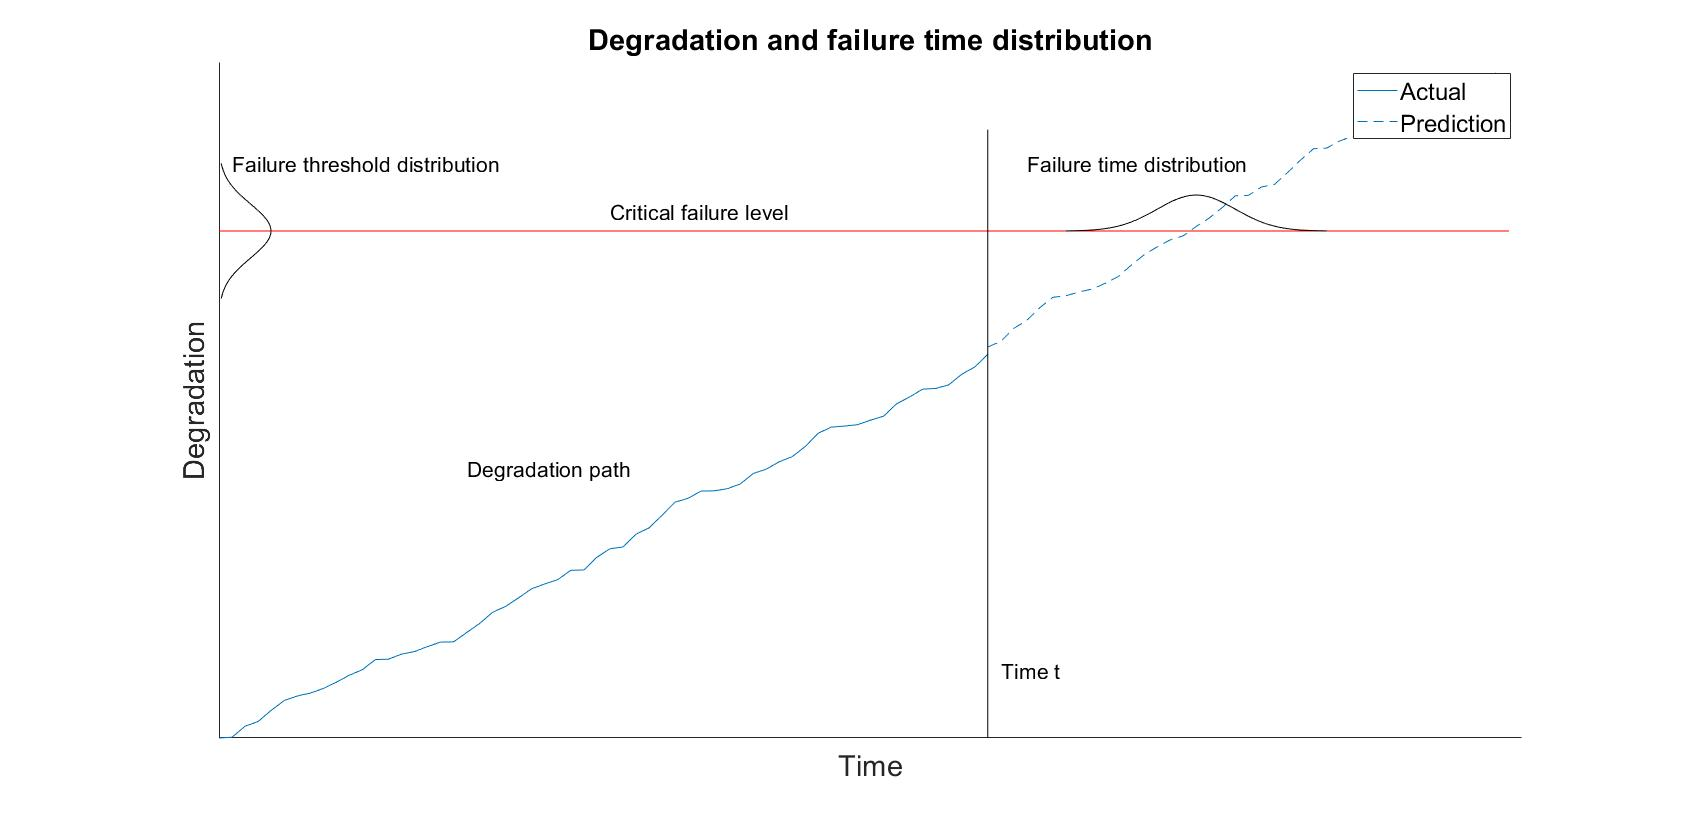
\includegraphics[width=\textwidth]{Figures/DegradationDistribution}
\caption[Degradation path and failure time distribution]{Degradation path and failure time distribution} \label{fig:DegradationDistribution}
\end{figure}

\subsection{Degradation path} \label{Degradation path}
As concluded from Section \ref{Position Error}, degradation of a robot arm joint is indicated by the position error and therefore the position error is called degradation indicator (DI). The following definitions and notations are based on the ones used by \citet{Lu1993}. The DI evolves toward the critical degradation level, or failure threshold, corresponding to the moment when the robot arm joint is no longer able to perform its designated functions. For any time, reliability of the robot arm joint can be evaluated as the probability of the DI not overshooting the failure threshold. The DI path can be described by $y_i$ over time $t$, where $y_i$ is the $i$th joint's actual DI path $\eta_i$, a function of time, plus measurement error $\varepsilon_i$. In this case the DI path is related to the peak position error as described before. When more variables to describe degradation become available, for example temperature measurements, the DI path function can be adjusted by this future variables. For this research, the peak position error is the only parameter that is used to describe the DI. Time $t$ is the number of working days (all days minus weekends and vacations). $M$ is used to denote the failure threshold. The failure time $T$ is defined as the time when the actual path $\eta$ crosses failure threshold $M$. The DI path of the $i$th robot arm joint at time $t_j$ is given by 
\begin{equation} \label{eq:degradation path}
\begin{aligned} 
	y_{ij} & = \eta_{ij} + \varepsilon_{ij} = \eta(t_j) + \varepsilon_{ij},& i & =1,2,\ldots,n, \\    
    \varepsilon_{ij} & \sim N(0,\sigma^{2}_{\varepsilon}),& j & =1,2,\ldots,m_i,
\end{aligned}
\end{equation}
where $t_j =$ time of the $j$th measurement; $\varepsilon_{ij}=$ measurement error with  standard deviation $\sigma_{\varepsilon}$; $\eta_{ij}=$ actual DI path of the $i$th joint at time $t_j$; $m_i=$ total number of inspections of the $i$th joint. \citet{Lu1993} describe that $\eta_{ij}$ has fixed and random-effect parameters denoted by $\Phi$ and $\Theta_{i}$. However, for this project it is assumed that the peak position error can indicate robot failure only and therefore $\eta_{ij}$ only consist of one parameter; peak position errors.

To give an idea how the DI path evolves in time, an example is provided in Figure \ref{fig:RB72R1J1Degradation}. It can be seen that the DI, or peak position error, increases slowly over time, on average. After the high peak around the $18$th monitored working day, it was replaced by a revised one. From here it can be seen that the DI for the revised robot arm, that execute the same task as the old one, is lower. The replaced robot arm was in operation for more than 3 years, or approximately 780 working days. The monitoring time, 25 working days, is too small to conclude anything about the actual DI path the arm underwent and assumptions have to be made. It is therefore assumed that robot arm joints degrade linearly.
\begin{figure}[ht]
\centering
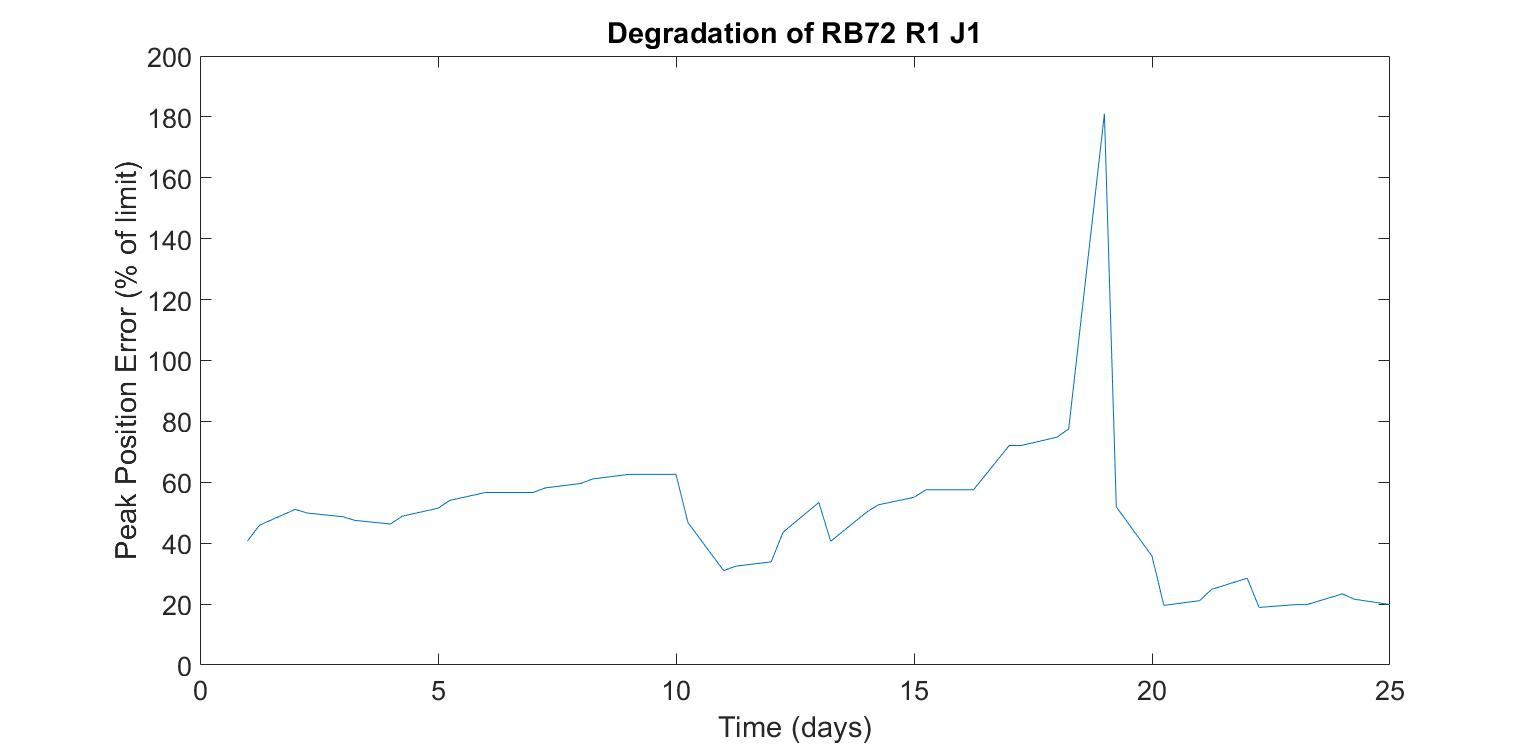
\includegraphics[width=\textwidth]{Figures/RB72R1J1Degradation}
\caption[Degradation path of RB72 Robot1 Joint 1]{Degradation path of RB72 Robot1 Joint 1} \label{fig:RB72R1J1Degradation}
\end{figure}

\subsection{Time to failure estimation} \label{TTF}
In this research the time to failure (TTF) is defined as the time between the last observation and the failure time T with respect to the degradation path. The TTF can be considered as a random variable with a probability distribution. A robot arm joint is considered to be failed when the DI cross a failure threshold, specified in the next section \ref{Random threshold}. The probability distribution function of TTF is denoted by $F_{TTF}$ is defined as follows:
\begin{equation} \label{eq:TTFeq:TTF}
F_{TTF}(t_j)=Pr[TTF \leq t_j] = \frac{1}{\sqrt[]{2\pi\sigma^2}} \int\limits_{-\infty}^{t_j} \mathrm{e}^{\frac{-(t_j-\mu)^2}{2\sigma^2}}
\end{equation}
In other words, $F_{TTF}(t_j)$ is the probability that a failure occurs in the interval $(-\infty,t_j]$ with normal distribution parameters $\mu$ and $\sigma$. This PDF is used to provide a relative likelihood that the value of the DI path will cross the threshold. 

Increments are defined as the discretized increase or decrease of the DI during a day. Since that the increments can be either positive or negative, a normal distribution is considered depicted in Figure \ref{fig:RB72R1J1PDF} for RB72 Robot1 Joint1 with $\mu=0.098292$ and $\sigma=6.4403$. Data that is used to obtain those values can be found in Appendix REF. Here, $\chi$ is the positive or negative increment size over which the peak position error can evolve per day. The obtained PDF will be different for every robot arm, since the size and frequency of increasing and decreasing position error increments will differ per arm. For this project, a fixed number of inspections is used to build the PDF and estimate a DI path prediction. However, updating the PDF is necessary to make the model more dynamic and adaptive to new input data. How this is intended will be described in Chapter \ref{Chapter6}.

\begin{figure}[ht]
\centering
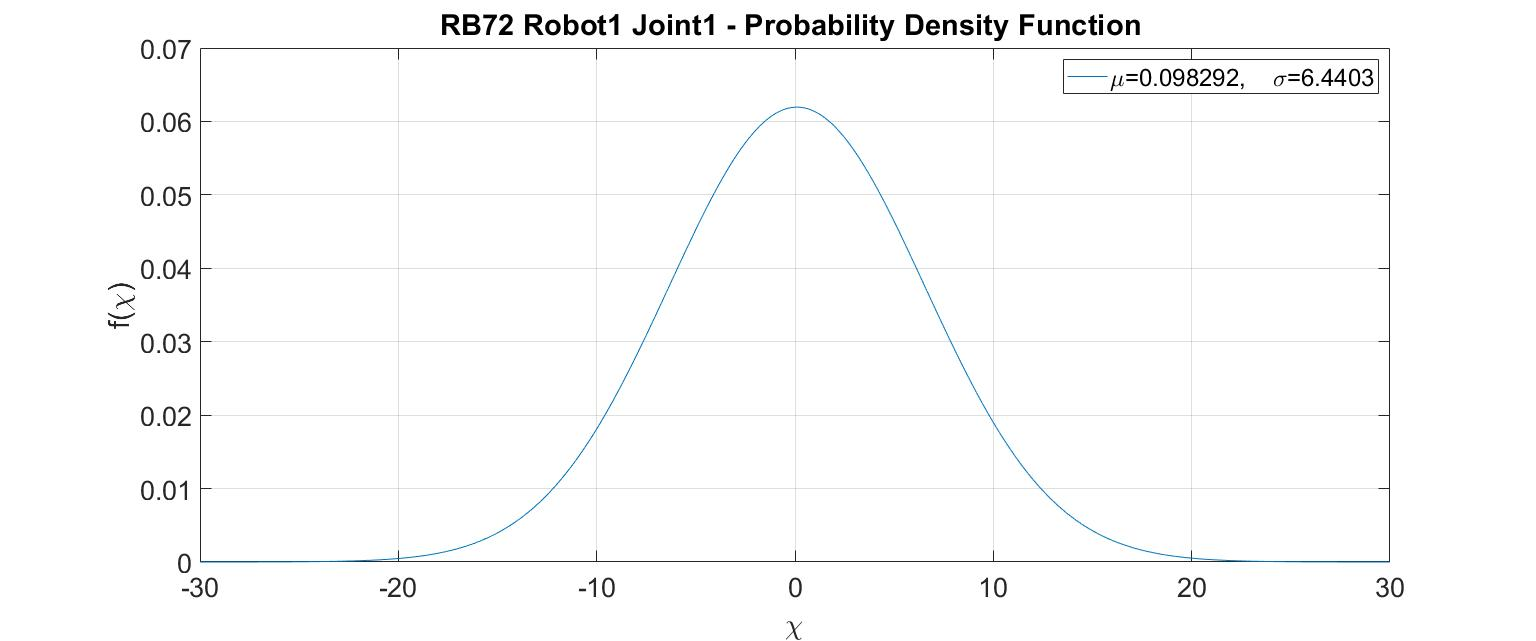
\includegraphics[width=\textwidth]{Figures/RB72R1J1PDF}
\caption[Probability density function of RB72 Robot1 Joint 1 degradation]{Probability density function of RB72 Robot1 Joint 1 degradation} \label{fig:RB72R1J1PDF}
\end{figure}

\subsection{Random deviations in failure threshold} \label{Random threshold}
\citet{Usynin2008} describe that most models used in degradation data analysis make use of the notion of a fixed critical failure threshold, in this case denoted as $M$. Since, joint failures occur at different DI values (position errors), see Section \ref{Position Error}, a probabilistic description is likely to be more appropriate. The failure threshold differs per robot and therefore a PDF that reflects the relatively vague knowledge about possible failure thresholds is used. In this case, failure threshold $M$ is defined as a range of critical values having certain probabilities. 

The following definitions and notations are based on \citet{Usynin2008}. Let $F_{M}(y)$ be the cumulative distribution function of the random critical failure threshold.
\begin{equation} \label{eq:CDF}
F_{M^*}(y)=Pr[M^*< y]
\end{equation}
where $M^*$ is the random failure threshold for degradation $y$.
\begin{equation}
f_{M^*}(y) = \frac{dF(y)}{dy}
\end{equation}
is the probability density function of the random failure threshold $M^*$. 

Only from RB72 Robot1 Joint1 and RB34 Robot2 Joint1 it is known what their failure threshold is, 70 and 25 respectively. Therefore, this PDF is constructed based on the researchers intuition and knowledge about failure levels. TBD

%Robot arms exhibit very complex dynamic behavior, and different defects can affect this behavior. Also, their motion is completely different from that of rotating machines (or other continuously moving machines), for which the majority of present condition monitoring systems have been designed. \citet{Jaber2017} describes that data subtracted from a robot arm are transitory and last for a very short time. This is in contradiction with the rotating machines discussed widely in literature that emit continuous signals during their operation. The challenge here is how to design a reliable and intelligent condition monitoring system to be able to deal with the transitory and non-transitory signals for accurate diagnosis and prognosis.Therefore, the signals captured and features extracted have to be analyzed and classified in an appropriate way to provide an unambiguous identification of a faulty robot part before a catastrophic failure occurs.

%Currently, the OTD of Philips uses direct inspection to measure the condition of robot arms and to find defective faults. By applying CBM, these direct inspections should be replaced by condition monitoring using sensors within the robot arm. In Section \ref{SQ1}, it is determined what data types should be analyzed to achieve a reliable maintenance prediction. 

\section{SQ3: On what performance indicators should the artifact be evaluated?} \label{SQ3}
The DI path $y$ \ref{eq:degradation path} and probability density functions $f_{M^*}$ \ref{eq:CDF} and $F_{T}$ REF should be checked on their correctness. Since the monitoring time of the robot arms is relatively small, as discussed in the previous section, a simulation is performed besides an experiment to check the appropriateness of the PDF based model. 

\subsection{Experiment} \label{Experiment}
In this section, the model is tested on new real experiment data available from robot arms to check whether the model is able to determine when it will cross the failure threshold. Data available 

\subsection{Simulation} \label{Simulation}
By performing simulations, the model can be tested how it will contribute to the maintenance schedule at Philips. 

\subsection{Comparison of experiment and simulation} \label{ExpvsSim}
The results of the experiment and the simulation will be discussed and compared.

\section{SQ4: What are requirements for software engineers to integrate the artifact in the control system?} \label{SQ4}
The validated model should be implemented into the RB34 and later in other RACs and therefore software requirements should be determined. Maybe a conversation with Frank Velthuis, a software engineer from Beenen, will bring some new insights forward. TBD
